\section{Evaluation}
\label{sec:eval}

\Mar{I think the high-level goal should be something along the lines
  of understanding prevalence of long test runs and main sources of
  cost in open-source Java projects.  Intuitively, the problem should
  come before the solution :).  Based on that, we study
  parallelization of testing frameworks.  More precisely, we
  investigage how prevalent test parallelization is, the potential for
  improving execution cost, issues of flakiness that hinders use of
  parallelization, and how to address those issues.}

We evaluated the characteristics of regression tests in open-source
development from a sample set of Java projects from Github. We are
interested in understanding the prevalence of long test runs, the main
sources of cost, and how do developers explore parallelism to improve
execution performance. More specifically, we pose the following
research questions:

\newcommand{\RQA}{How prevalent is the occurence of time-consuming
regression test suites in open-source projects?}
\newcommand{\RQB}{How often are parallelization features present in
build files?}
\newcommand{\RQC}{What is the impact of parallalelization?}

\newcommand{\RQD}{What factors contribute to improve performance
through parallelization?\Jbc{Previously as "When does parallelization
works and when it does not so great?"}}

\newcommand{\RQE}{What are the limitations of parallelization?}

\newcommand{\rqOne}{\textbf{RQ1.} \RQA}
\newcommand{\rqTwo}{\textbf{RQ2.} \RQB}
\newcommand{\rqThree}{\textbf{RQ3.} \RQC}
\newcommand{\rqFour}{\textbf{RQ4.} \RQD}
\newcommand{\rqFive}{\textbf{RQ5.} \RQE}

\begin{itemize}
    \item \rqOne
    \item \rqTwo
    \item \rqThree
    \item \rqFour
    \item \rqFive
\end{itemize}

%%\newcommand{\RQB}{What is the distribution of CPU and IO bound
%%regression test suites from the sample set?}
%%
%%\newcommand{\RQC}{How uniformly distributed is the execution time
%%across test cases in costly projects?}
%%
%%\newcommand{\RQD}{How often developers use the parallelism features
%%from build systems to improve runtime performance?}

The first research question addresses the prevalence of long-running
test suites. We are interested to know if costly test suites are
common in open-source projects.  The second research question
addresses our interest in understanding if developers are aware of
parallelization features from testing frameworks available
out-of-the-box through build systems (\eg, run JUnit test cases in
parallel using Maven Surefire) and what setting are more often used.
The third research question addresses the impact of parallelism on the
regression tests from our sample set. We are interested in compare the
execution performance with different parallel settings (see
Section~\ref{sec:modes}). The fourth research question addresses the
characteristics of regression tests from the previous experiment.
More specifically, we want to investigate if there is a relation
between the balance of test execution (\ie, how uniformly distributed
is the execution time across tests cases) and the usage of
computational resources (\ie, if tests are mostly CPU or IO intense)
that impacts the effectiveness of parallelization. Finally, the fifth
research question discusses the limitations and insights to overcome
the pitfalls of parallelization.

\Comment{
    \Fix{distribution of execution time per test case. For each subject
    identified in the first research question, we investigate how
    balanced is the cost of the test suite in contrast to the cost of
    test cases and if there are subjects where the time cost is mostly
    dominated by a small fraction of test cases.} \Fix{The third research
    question addresses the distribution of regression tests according
    to the use of computational resources.  We are interested in
    investigating if regression test suites are CPU intensive and if there
    are opportunities to improve performance. The RQ4 addresses}
    \Fix{...elaborate...}

    The rationale is that if the time cost of a regression test is equally
    distributed among test cases, the execution cost could be potentially
    improved by running tests in parallel (in contrast to the scenario
    where only one test case dominates most of the execution time).
}

\subsection{Subjects}
\label{sec:subjects}

We are interested to evaluate non-trivial test suites on popular
projects that are in activity. We used the Github's Search
API~\cite{githubsearch} to fetch Java projects according to the
following criteria: (1) the primary language must be Java\footnote{In
case of projects in multiple languages, the Github API considers the
predominant language as the primary language.}; (2) the project has at
least 100 stars; (3) latest update on (or after) January 1st, 2016;
(4) the \emph{readme} file contains the string \emph{mvn}.

On Github, when a user adds a star to a project, s/he demonstrated
appreciation and bookmarked it for later
reference~\cite{github-stars}.  Although there is not a specific range
for the number of stars, our criteria is an estimation to avoid
trivial subjects: we assumed that Github users are likely to
demonstrate interest on well-tested projects. The third criteria is a
constraint to skip projects without recent activity. The fourth
criteria is an approximation to find projects with Maven support. We
used Maven as a reference due to its popularity on Java projects and
to automate our evaluation scripts. The rationale is that if the
string \emph{mvn} exists in the \emph{readme} file, it may represent a
Maven call (\eg, to compile or test the project).
Figure~\ref{fig:subject-query} illustrates the query as an HTTP
request.

\begin{figure}[h!]
\centering
\scriptsize
\lstset{
    escapeinside={@}{@},
    numbers=left,xleftmargin=1em,frame=single,framexleftmargin=0.5em,
    basicstyle=\ttfamily\scriptsize, boxpos=c, numberstyle=\tiny,
    deletekeywords={true}
}
\begin{lstlisting}
https://api.github.com/search/repositories?q=
    stars:>=100+language:java+mvn%20in:readme+
    pushed:>=2016-01-01+sort:stars

\end{lstlisting}
\caption{\label{fig:subject-query} Query to the Github API for
    projects with the following criteria: (1) Java, (2) at least 100
    stars, (3) updated on January 1st, 2016 (or later), (4) contains
    the string \emph{mvn} in the \emph{readme} file. Output is
    paginated in descending order of stars.}
\end{figure}

A Maven project may contain several submodules with multiple
\emph{pom.xml} files. We considered only projects with a
\emph{pom.xml} file located in the root directory.  As of December
30th 2016, our search criteria returned 615 subjects. From the 615
downloaded projects, 46 were not Maven projects, 27 were unable to
fetch all dependencies (\eg, due to the usage of a private library),
and 131 were in an unstable revision. Our final set consists in
\numSubjs{} subjects.

\subsection{Setup and Replication}
\label{sec:setup}

To run our experiments, we used a \emph{Core i7-4790} (3.60 GHz) Intel
processor machine with 8 virtual CPUs (4 cores with 2 native threads
each) and 16GB of memory, running \emph{Ubuntu 14.04 LTS Trusty Tahr}
(64-bit version). Software settings include \Comment{the Linux
\emph{sysstat} package to measure performance, }\emph{git} to fetch
subjects, \emph{Java 8} and \emph{Maven 3.3.9} to build and test subjects,
and \emph{Python 3.4} to run our evaluation scripts. For replication,
all source artifacts are publicly available at \Fix{create gh-pages},
including supporting scripts (\eg, the script that test subjects and
generates the raw data), and the full list of projects. \Comment{, and a
\emph{Vagrantfile} to emulate our hardware and all software
dependencies.}

\subsection{Answering research question RQ1}
\label{sec:rqone}

\begin{itemize}
    \item \emph{\RQA}
\end{itemize}

To evaluate the frequency of time-consuming regression tests, we
considered the \numSubjs{} subjects from Section~\ref{sec:subjects} and
compared the elapsed time to run their tests.
Figure~\ref{fig:mvn-execution} shows the commands used in our script
to test each subject. The main loop (lines 6-12) iterates over the
list of subjects and invokes Maven in separated steps (lines 8-10). To
avoid inflating the measured time, we first compile the source and
test files (line 8), fetch all dependencies (line 9) and later, we run
the tests in offline mode (line 10) to avoid package updates. In
addition we randomly selected 100 Maven logs to inspect and identify
non-related tasks (\eg, \emph{javadoc} generation and static
analysis). We created a list of plugins (lines 1-4) to ignore them
during the test execution.  Finally, we use a simple regular
expression over the test output to extract the elapsed time (line 13).
We executed this experiment \Fix{X} times in our dedicated server
remotely via SSH with the operating system running only essential
services (\eg, the SSH server).

\begin{figure}[h!]
\centering
\scriptsize
\lstset{
    escapeinside={@}{@},
    numbers=left,xleftmargin=1em,frame=single,framexleftmargin=0.5em,
    basicstyle=\ttfamily\scriptsize, boxpos=c, numberstyle=\tiny,
    showstringspaces=false
}
\begin{lstlisting}[language=Bash]
MAVEN_IGNORES="-Dmaven.javadoc.skip=true \
    -Drat.skip=true -Djacoco.skip=true \
    -Dcheckstyle.skip=true -Dfindbugs=true \
    -Dcobertura.skip=true"

for subj in ${SUBJECTS}; do
    cd ${SUBJECTS_HOME}/${subj}
    mvn clean install -DskipTests ${MAVEN_IGNORES}
    mvn dependency:go-offline
    mvn -o test ${MAVEN_IGNORES} &> ${LOG}
    cat ${LOG} | grep "\[INFO\] Total time:"
done
\end{lstlisting}
\caption{\label{fig:mvn-execution} Bash script to evaluate the time cost of
    test suites. For each subject, we compile the source and test files, fetch
    all dependencies, and execute the tests in offline mode ignoring
    non-related tasks. Unnecessary commands are omitted for simplicity.}
\end{figure}

We grouped the subjects according to the execution time: tests that
ran in less than one minute (\emph{short execution}), one to five
minutes (\emph{medium execution}), and more than five minutes
(\emph{long execution}). A previous work used a similar categorization
except for the \emph{medium} group \cite{gligoric-etal-issta2015}.  We
added a new group because \Fix{justify or use the same
classification}.  Figure~\ref{fig:piechart-time} shows the proportion
of subjects per group and Figure~\ref{fig:boxplots-time} shows the
distribution of elapsed time for each group (boxplots).

\begin{figure}[h!]
    \centering
    \begin{minipage}{2in}%
    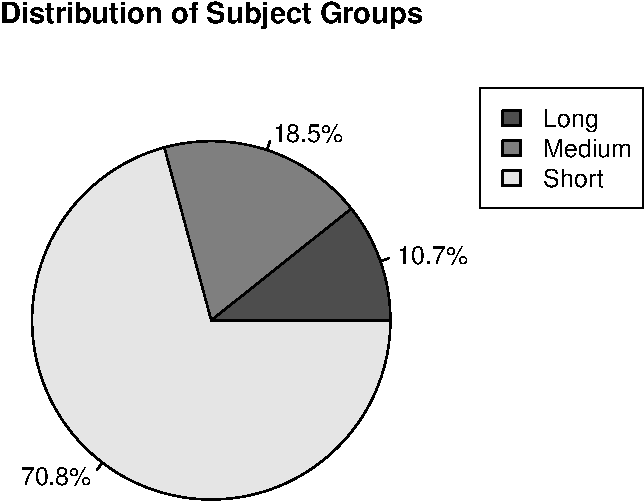
\includegraphics[width=\textwidth]{plots/piechart-timecost.pdf}
    \end{minipage}%
    \caption{\label{fig:piechart-time} Subjects grouped by elapsed time on test
    execution ($t$): short execution ($t < 1m$), medium execution ($1m \leq t <
    5m$), and long execution ($5m \leq t$).}
\end{figure}

\begin{figure}[h!]
    \centering
    \begin{minipage}{2.5in}%
    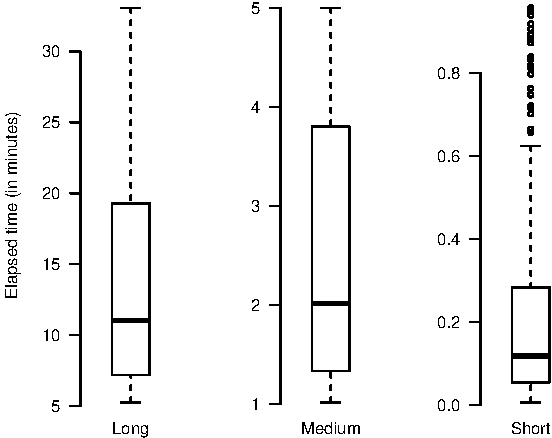
\includegraphics[width=\textwidth]{plots/boxplots-timecost.pdf}
    \end{minipage}%
    \caption{\label{fig:boxplots-time} Distribution of time execution
    per group. Outliers from \emph{Long} are ignored for better
    readability.}
\end{figure}

Results indicate that a relatively high number of projects from the
sample set (\ie, 29,2\%) requires at least five minutes to execute.
The boxplot for the \emph{long} group reveals \Fix{dissect the
boxplot: skewness, median, IQR}. \Fix{Discuss outliers from Long
group}.  It is important to mention that
Figure~\ref{fig:piechart-time} represents a lower bound for elapsed
time: some tests may finish early due to a failure since the subjects
were tested in a potentially unstable revision.

\subsection{Answering research question RQ2}
\label{sec:rqTwo}

\begin{itemize}
    \item \emph{\RQB}
\end{itemize}

To evaluate the presence of parallelization settings, we considered
the \Fix{91} subjects from the groups \emph{long} and \emph{medium}
identified in Section~\ref{sec:rqone}. We focused in these two groups
because they represent costly test suites and are more likely that the
developers may have used strategies to reduce the execution cost (\eg,
running parts of the tests in different threads). We computed the
frequence of the parallelism modes (see Section \ref{sec:modes}) using
a semi-automatic approach: we first discover automatically the
relevant configuration files and then we manually inspect them to
eliminate false-positves (\eg, commented configuration).  Figure
\Fix{N} describes the discovery step. We first list the paths of all
build file and then we filter only the build files that contain any of
the keywords, \CodeIn{forkMode}, \CodeIn{forkCount}, or
\CodeIn{parallel}.

\begin{figure}[h!]
\centering
\scriptsize
\lstset{
    escapeinside={@}{@},
    numbers=left,xleftmargin=1em,frame=single,framexleftmargin=0.5em,
    basicstyle=\ttfamily\scriptsize, boxpos=c, numberstyle=\tiny,
    showstringspaces=false
}
\begin{lstlisting}[language=Bash]
for subj in ${SUBJECTS}; do
    subject_path=${SUBJECTS_HOME}/${subj}
    build_files=`find $subject_path -name pom.xml`
done
\end{lstlisting}
\caption{\label{fig:discovery-step} Bash script \Fix{to do
         something...}. Unnecessary commands are omitted for simplicity.}
\end{figure}

\Fix{---------------------}


In an initial exploration, we searched for
evidences of low-level parallelism settings on configuration files
(\ie, \emph{pom.xml}) from each subject using a semi-automated
approach: we use a script to find all subjects with evidences of
parallel settings and then we manually inspect each configuration file
to eliminate false-positives. In addition, we are interested in
understanding how these parallel settings are used. Given a list of
subjects, our script searches recursively all \emph{pom.xml} files
from the project directory and uses the command-line tool \emph{grep}
to highlight the presence of the keywords \emph{forkMode},
\emph{forkCount}, and \emph{parallel}.  Any of these keywords exist in
any possible combination of parallel settings (see
Section~\ref{sec:modes}). From the 91 subjects, our script detected 43
subjects with evidence of parallel settings. After the inspection of
130 configuration files, we confirmed that \Fix{X} settings are real
parallel configurations.  These settings are related to \Fix{Y}
subjects. It is important to notice that, \Fix{X}\% of the subjects
(\emph{medium} and \emph{long} aggregated) did not explore low-level
parallelism according to our criteria of matching keywords. After the
inspection, this rate raises to \Fix{Y}\%. \Fix{elaborate: some
projects doesn't use parallel features, so what?}
Table~\ref{tab:inspection-table} summarizes our initial findings.

\begin{table}[h!]\footnotesize
    \centering
    \begin{tabular*}{0.5\textwidth}{cccc}
        \toprule
        Group  & Subjects with Evidence & Config. Files & Config. Confirmed\\
        \midrule
        Long   & 22 / 35    & 77 / 1981       & \Fix{X} / 77\\%
        Medium & 21 / 56    & 53 / 491        & \Fix{X} / 53\\%
        \midrule 
        Total  & 43 / 91    & 130 / 2472      & \Fix{X} / 130\\
        \bottomrule
    \end{tabular*}
    \caption{\Fix{to-be-defined}}
    \label{tab:inspection-table} 
\end{table}



\Fix{elaborate: write about the subjects that use parallelism - How do
they use them? Would it be possible to measure the benefits? How the
configs from Section~\ref{sec:modes} are distributed?}

%%To evaluate the distribution of execution time per project, we sorted
%%the test cases by decreasing order of elapsed time and calculated the
%%number of tests executed in 90\% of the total time. Later, we reported
%%the \Fix{balance} of execution time by dividing the number of tests
%%that represents 90\% of the execution time by the number of tests
%%cases. For instance, a balance of 50\% indicates \Fix{...}.  \Fix{We
%%collected the elapsed time from test cases for each generated report.
%%Maven Surefire generates an XML report with execution information
%%(\eg, number of skipped tests and elapsed time) per test suite
%%\Jbc{Should I use the previous sentence as a footnote or should I
%%delete it?}. We noticed that some test cases reported an elapsed time
%%of zero: since the reported time is in milliseconds, some tests may
%%execute in a shorter time. \Fix{..to be continued...}}. Results
%%indicate that \Fix{...}.
%%
%%\begin{figure}[h!]
%%    \centering
%%    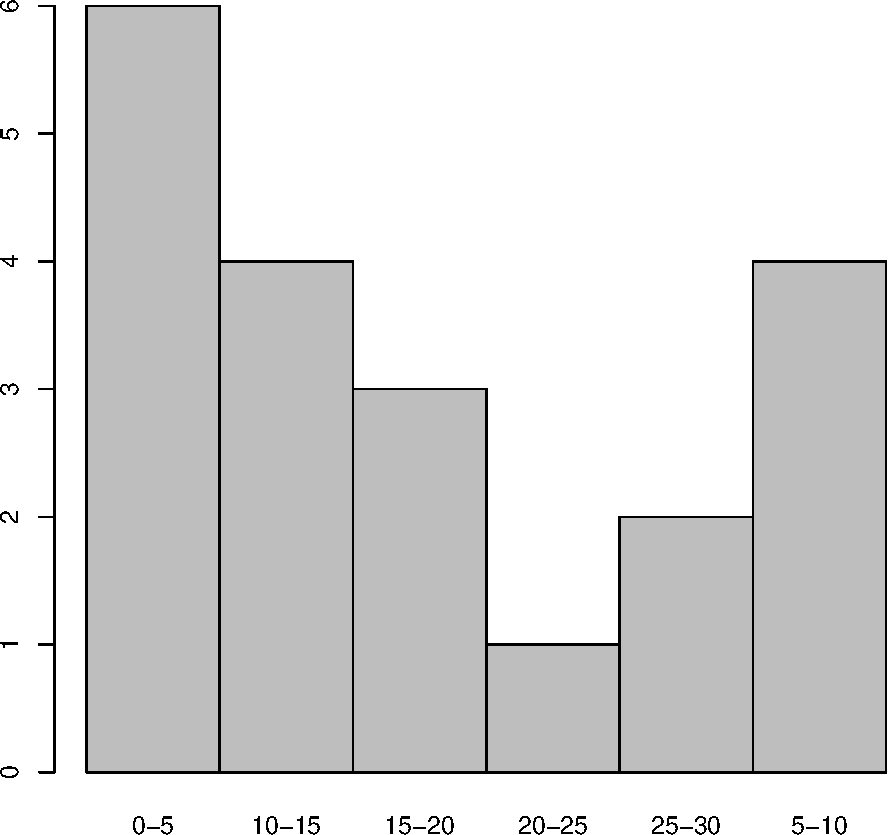
\includegraphics[width=0.4\textwidth]{results/plots/balance.pdf}
%%    \caption{\Fix{balance}}
%%\end{figure}

%% \subsection{Answering research question RQ3}
%% \label{sec:rqThree}
%% 
%% \begin{itemize}
%%     \item \RQB
%% \end{itemize}
%% 
%% To evaluate the distribution of CPU and IO intensive test suites from
%% the sample set, we used the command \emph{sar} to monitor the system
%% activity in background while tests ran. \emph{Sar} is a command that
%% collects and reports statistics (\eg, percentage of IO waiting and
%% usage of CPU in user mode) based on the kernel activity and it is
%% highly configurable to collect detailed information (\eg, usage of a
%% specific processor core or percentage of network interface
%% utilization). We configured \emph{sar} to report \Fix{...explain how
%% we executed and what fields we are interested}. \Fix{explain fields}.
%% Figure \Fix{A} shows the distribution of subjects grouped in intervals
%% of \Fix{W}\% of CPU utilization. Results indicates that \Fix{...}
%% 
%% \begin{figure}[h!]
%%     \centering
%%     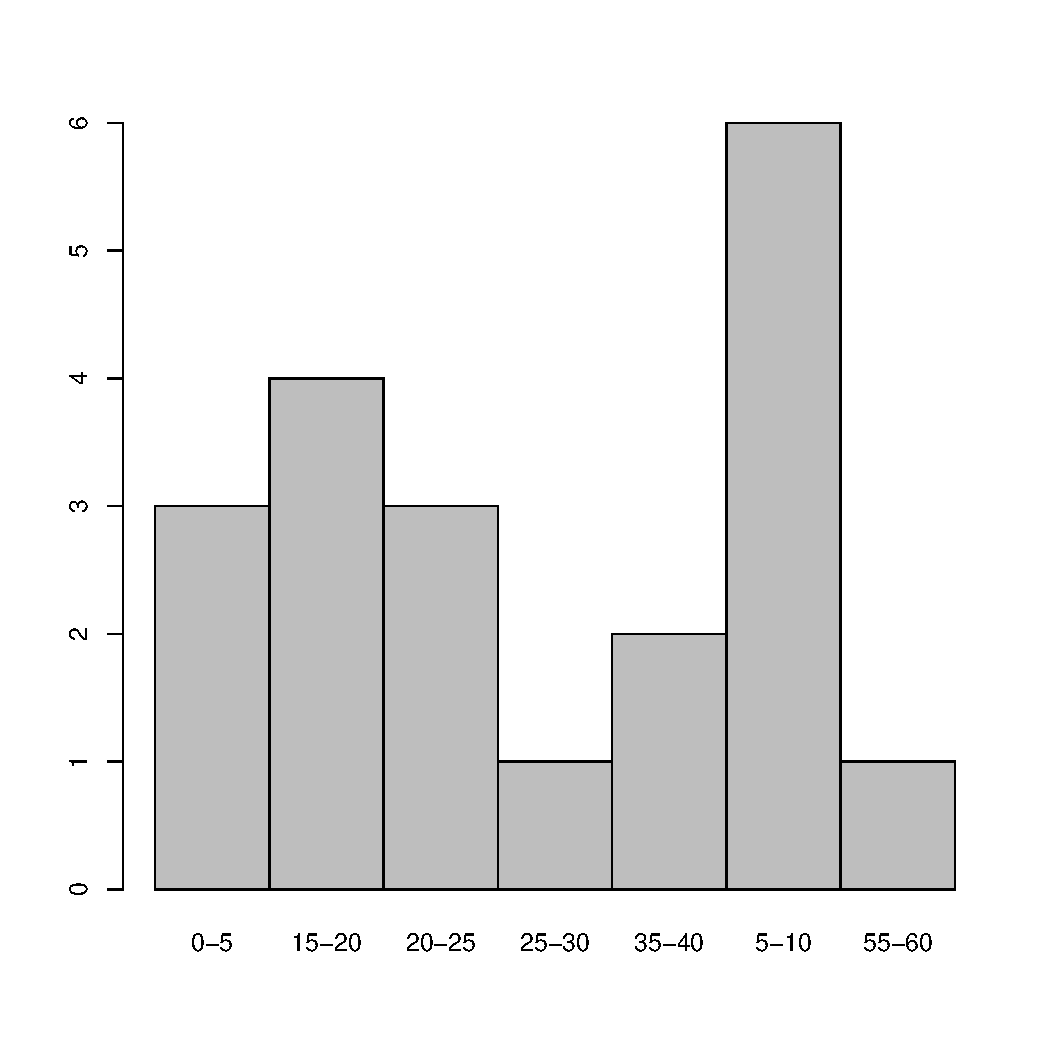
\includegraphics[width=0.4\textwidth]{results/plots/cpuness.pdf}
%%     \caption{\Fix{cpu usage}}
%% \end{figure}
%% 
%% \Comment{we proposed the definition of \emph{cpuness}
%% computed as the follow: $((user\_t + system\_t) / elapsed\_t) * 100$,
%% where \emph{user\_t} is the elapsed time of execution in \emph{user
%% mode}, \emph{system\_t} is the elapsed in \emph{kernel mode}, and
%% \emph{elapsed\_t} is the elapsed time to finish the execution. We
%% measured the \emph{cpuness} of each regression test \Fix{...elaborate
%% the meaning of cpuness} \Fix{Describe how I measured user, system and
%% "wall" time}.  \Fix{Explain results}.  \Fix{show plots}}
%% 
%% \subsection{Answering research question RQ4}
%% \label{sec:rqfour}
%% 
%% \begin{itemize}
%%     \item \RQD
%% \end{itemize}
%% 
%% \Fix{to appear...}
%% 
